% Autor: Leonhard Segger, Alexander Neuwirth
% Datum: 2017-10-30
\documentclass[
	% Papierformat
	a4paper,
	% Schriftgröße (beliebige Größen mit „fontsize=Xpt“)
	12pt,
	% Schreibt die Papiergröße korrekt ins Ausgabedokument
	pagesize,
	% Sprache für z.B. Babel
	ngerman
]{scrartcl}

% Achtung: Die Reihenfolge der Pakete kann (leider) wichtig sein!
% Insbesondere sollten (so wie hier) babel, fontenc und inputenc (in dieser
% Reihenfolge) als Erstes und hyperref und cleveref (Reihenfolge auch hier
% beachten) als Letztes geladen werden!

% Silbentrennung etc.; Sprache wird durch Option bei \documentclass festgelegt
\usepackage{babel}
% Verwendung der Zeichentabelle T1 (Sonderzeichen etc.)
\usepackage[T1]{fontenc}
% Legt die Zeichenkodierung der Eingabedatei fest, z.B. UTF-8
\usepackage[utf8]{inputenc}
% Schriftart
\usepackage{lmodern}
% Zusätzliche Sonderzeichen
\usepackage{textcomp}

% Mathepaket (intlimits: Grenzen über/unter Integralzeichen)
\usepackage[intlimits]{amsmath}
% Ermöglicht die Nutzung von \SI{Zahl}{Einheit} u.a.
\usepackage{siunitx}
% Zum flexiblen Einbinden von Grafiken (\includegraphics)
\usepackage{graphicx}
% Abbildungen im Fließtext
\usepackage{wrapfig}
% Abbildungen nebeneinander (subfigure, subtable)
\usepackage{subcaption}
% Funktionen für Anführungszeichen
\usepackage{csquotes}
% Zitieren, Bibliographie
\usepackage{biblatex}

% Verlinkt Textstellen im PDF-Dokument
\usepackage[unicode]{hyperref}
% "Schlaue" Referenzen (nach hyperref laden!)
\usepackage{cleveref}
% Zur Darstellung von Webadressen
\usepackage{url}
%chemische Formeln
\usepackage[version=4]{mhchem}
% siunitx: Deutsche Ausgabe, Messfehler getrennt mit ± ausgeben
\usepackage{floatrow}
\floatsetup[table]{capposition=top}
\sisetup{
	locale=DE,
	separate-uncertainty
}
%\bibliography{6Mi_S2_25-10-2017_References}

\begin{document}
	
	\begin{titlepage}
		\centering
		{\scshape\LARGE Versuchsbericht zu \par}
		\vspace{1cm}
		{\scshape\huge E5 - Magnetische Suszeptibilität\par}
		\vspace{2.5cm}
		{\LARGE Gruppe 6Mi \par}
		\vspace{0.5cm}
		
		{\large Alexander Neuwirth (E-Mail: a\_neuw01@wwu.de) \par}
		{\large Leonhard Segger (E-Mail: l\_segg03@uni-muenster.de) \par}
		\vfill
		
		durchgeführt am 08.11.2017\par
		betreut von\par
		{\large Fabian Schöttke}
		
		\vfill
		
		{\large \today\par}
	\end{titlepage}
	\tableofcontents
	\newpage
	
	\section{Kurzfassung}
	Die Reaktion eines Stoffes auf ein Magnetfeld wird durch die Volumensuszeptibilität $\chi_V$ beschrieben. Ein Stoff, der von einem Magneten abgestoßen wird, bezeichnet man als diamagnetisch ($\chi_V<0$) und als paramagnetisch, wenn er von ihm angezogen wird ($\chi_V>0$).

	Im ersten Versuch wurden die Oberflächenformen von Flüssigkeiten durch einen Neodymmagneten verändert und mithilfe einer Fermi-Abschätzung ihrer magnetischen Suszeptibilität beurteilt.
	Als nächstes bestimmten wir die magnetischen Volumensuszeptibilitäten von Glas, Aluminium und Graphit indem wir den Unterschied der Gewichtskraft von einer Probe im Magnetfeld und einer ohne Magnetfeld betrachteten. 
	Zuletzt wurde noch die Reaktion von Aluminium auf einen bewegten Magneten untersucht.
	Zusammengefasst sind unsere Ergebnisse, dass Glas, Graphit und Wasser diamagnetisches Verhalten aufweisen. Aluminium und Mangan-Chlorid-Lösungen reagieren paramagnetsich. Des Weiteren sind die paramagnetischen Effekte des Aluminiums gegenüber Induktionseffekten vernachlässigbar. 
	
	\section{Fermi Abschätzung zum Einfluss der Suszeptibilität auf die Oberflächenform einer Flüssigkeit}
	\subsection{Methoden}
	Es ist zu erwarten, dass eine diamagnetische Flüssigkeit über einem Magneten ein Tal ausbildet, weil sie vom Magneten abgestoßen wird, und eine paramagnetische einen Berg ausbildet, weil sie in den Bereich über dem Magneten gezogen wird. %Er hat das dritte Komma durchgestrichen, aber man darf da ein Komma setzen.
	Um gemäß dieses Zusammenhangs Rückschlüsse auf die Suszeptibilität von Flüssigkeiten zuzulassen, wurde ein Laser auf eine Flüssigkeit in einer Petrischale gerichtet und die Reflexion des Lasers auf einer Wand beobachtet. Dann wurde vom Versuchsbetreuer unter der Petrischale ein Magnet hindurch bewegt. Aus der Änderung des Reflexionswinkels lässt sich dann die Höhe des Tals oder Berges über dem Magneten abschätzen. Untersucht wurde Wasser und mit Wasser verdünntes Mangan(II)-chlorid.
	\subsection{Ergebnisse}
	Bei Breite des Magneten $d \approx \SI{1}{cm}$, Ruhelage der Reflexion auf der Wand $b \approx \SI{3}{m}$ und Abstand der Petrischale zur Wand $a \approx \SI{6}{m}$ haben wir für die Auslenkung $\Delta y$ des Lasers auf der Wand: \newline
	\begin{gather*} 
		\Delta y_\text{\ce{H2O}} \approx \SI{-7}{cm} \\
		\Delta y_\text{\ce{MnCl2}} \approx \SI{15}{cm}
	\end{gather*}
	abgeschätzt.
	Zur Näherung der Verformung der Wasseroberfläche nutzen wir eine Fermi-Abschätzung. Dafür treffen wir die vereinfachende Annahme, dass der Berg bzw. das Tal eine Dreiecksform haben, mit dem Ziel, die Höhe $y_\text{S}$ des Dreiecks zu bestimmen. Zugrunde legen wir das Reflexionsgesetz für die Reflexion des Lasers an der Tal-/Bergwand.\\
	\cref{Fermi1}, \cref{Fermi2} und \cref{Fermi3} dienen der Erläuterung der Wahl unserer Variablen.
	\begin{figure}[htb]
	  \centering
	    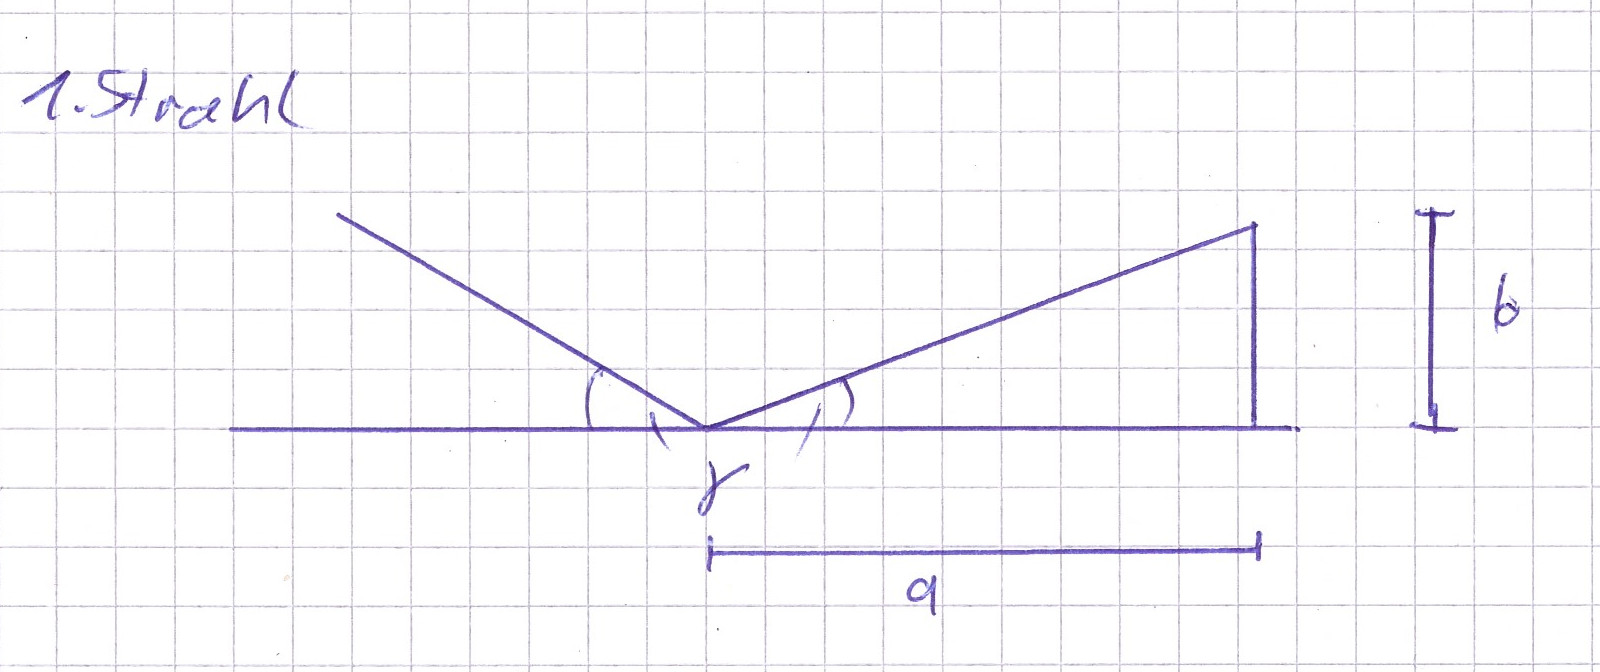
\includegraphics[width=0.6\textwidth]{Fermi1} 
		\caption[Fermi Abschätzung 1. Strahl Skizze]{Fermi Abschätzung 1. Strahl Skizze. Die Oberfäche der Flüssgkeit ist nicht unter Einfluss eines Magneten. $\gamma$ bezeichnet den Einfalls- sowie Ausfallswinkel zur Oberfläche und Horizontalen. $a$ und $b$ sind der Abstand zur Wand bzw. die Höhe des Laserslichts and der Wand.}

		\label{Fermi1}
	\end{figure}
	\begin{figure}[htb]
	  \centering
	    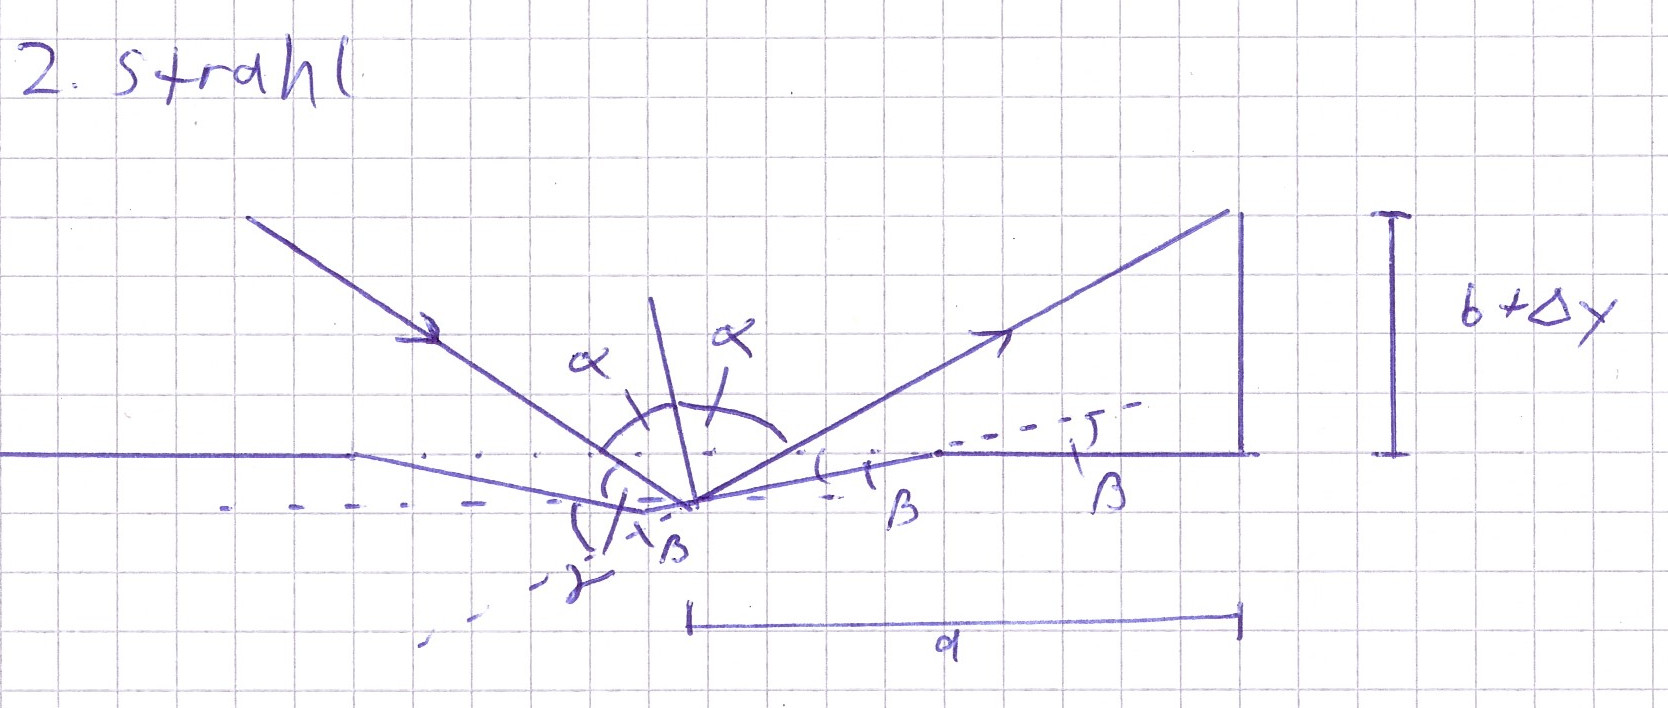
\includegraphics[width=0.6\textwidth]{Fermi2} 
		\caption[Fermi Abschätzung 2. Strahl Skizze]{Fermi Abschätzung 2. Strahl Skizze. Der Winkel $\beta$ bezeichnet den Winkel des Dreiecks der veränderten Oberflächenform der Flüssigkeit. $\gamma$ bezeichnet weiterhin den Winkel des einfallenden Lichtstrahls zur Horizontalen. Der Winkel des einfallenden, bzw ausfallenden Lichts zum senkrecht auf der Oberfläche stehenden Lot wurde als $\alpha$ bezeichnet.}
		\label{Fermi2}
	\end{figure}
	\begin{figure}[htb]
	  \centering
	    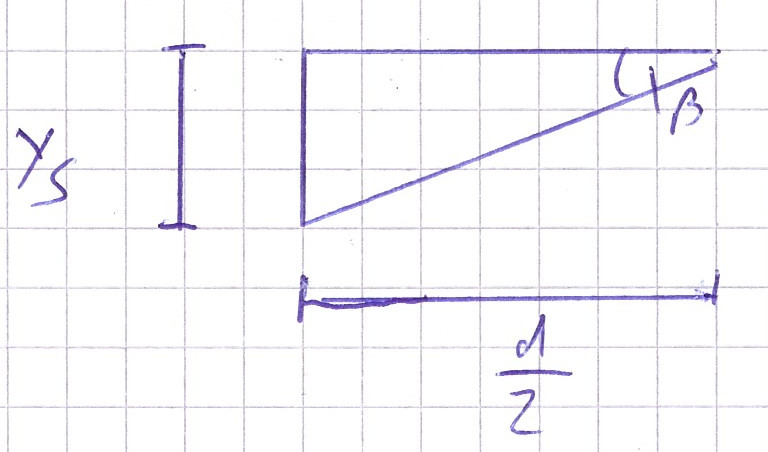
\includegraphics[width=0.6\textwidth]{Fermi3} 
		\caption[Fermi Abschätzung Dreieck Skizze.]{Fermi Abschätzung Dreieck Skizze. $y_S$ ist die vertikale Verscheibung der Oberfläche durch den Magneten.}
		\label{Fermi3}
	\end{figure}
	
	\noindent{}Berechnung des Einfallwinkels $\gamma$
	\begin{equation}
		\gamma = \arctan \left(\frac{b}{a}\right) 
		\label{gamma}
	\end{equation}
	Die Summe von $\alpha$ , $\beta$ und $\gamma$ ist der Winkel des Lots, das auf der gekrümmten Oberfläche steht
	\begin{equation}
		\alpha = \ang{90} - \beta - \gamma \\
		\label{alpha}
	\end{equation}
	Der Ausfallswinkel zur Horizontalen lässt sich bestimmen durch den Zusammenhang, dass $2\alpha + \gamma$ und der Ausfallswinkel genau $\ang{180}$ ergeben (\cref{Fermi2})
	\begin{equation}
		\arctan \left(\frac{b+\Delta y}{a}\right) = \ang{180} - \gamma - 2\alpha \\
	\end{equation}
	Durch Einsetzten von $\alpha$ aus \cref{alpha} erhält man
	\begin{equation}
		\arctan \left(\frac{b+\Delta y}{a}\right) = \gamma + 2 \beta \\
	\end{equation}
	Anwenden von \cref{gamma}
	\begin{equation}
		\arctan \left(\frac{b+\Delta y}{a}\right) =   \arctan \left(\frac{b}{a}\right) + 2 \beta \\
	\end{equation}
	Es folgt
	\begin{equation}
		\Rightarrow \beta = \frac{\arctan \left(\frac{b+\Delta y}{a}\right) -  \arctan \left(\frac{b}{a}\right)}{2} \\
	\end{equation}
	Nach \cref{Fermi3} ist
	\begin{equation}
		\Rightarrow y_\text{S} = \tan (\beta) \frac{d}{2}  
	\end{equation}
	Setzt man die gemessenen Werte in die Formel ein so erhält man: $ y_{\text{S,\ce{H2O}}} = \SI{-23}{\micro \meter} $ und $y_{\text{S,\ce{MnCl2}}} = \SI{49,5}{ \micro \meter} $. Das Wasser wird folglich abgestoßen und die Mangan-Chlorid-Lösung wird von dem Magneten angezogen.
	
	\subsubsection*{Zusätzliche Näherung:}
	Beim Aufstellen der Gleichung wurde die Approximation verwendet, dass beide Reflexionen in gleichem Abstand zur Wand stattfinden. Dass dies kaum Einfluss auf das Ergebnis nimmt, zeigt die folgende Rechnung: 
	\begin{align}
		\Delta x &= \tan (\gamma) y_\text{S} \\
		\Delta x &= \frac{b}{a} y_\text{S}
	\end{align}
	Da die Unsicherheit unserer Schätzung von $a$, bzw. von dem Verhältnis $\frac{b}{a}$, sehr viel größer als der Fehler $\Delta x_\text{S}$, der bei der Näherung entsteht, ist, ist der Beitrag von $\Delta x_\text{S}$ vernachlässigbar.

	\subsection{Schlussfolgerung}
	Das Wasser bildet über dem Magneten ein Tal in der Größenordnung von \SI{e-5}{m} aus. Dies lässt nach den obigen Überlegungen darauf schließen, dass Wasser diamagnetisch ist. Dies stimmt mit den Literatureigenschaften von Wasser überein.
	Manganchlorid hingegen bildet einen Berg der Größenordnung \SI{10}{\micro \meter} aus. Dies spricht für einen Paramagnetismus von in Wasser gelöstem Mangan(II)-chlorid. Auch dies entspricht den Literaturwerten für die magnetische Suszeptibilität von Mangan(II)-chlorid. Einen genaueren Rückschluss auf die Stärke der Verformung der Wasseroberfläche erlaubt dieser Versuch mit einer Fermi-Abschätzung nicht. Eine genauere Erfassung der Messgrößen und ein \enquote{Abrastern} der Oberfläche könnte jedoch ein recht präzises Bild der Wasseroberfläche erlauben. %TODO Quelle Wikipedia (mach ich noch)
	
	\section{Bestimmung der Volumensuszeptibilität von Glas, Aluminium und Graphit}
	\subsection{Methoden}
	Um die Volumensuszeptibilität von Glas, pyrolytischem Graphit und Aluminium zu bestimmen, haben wir die Änderung der Belastung einer Waage, auf der die Probe platziert wurde, mit und ohne Magneten darüber gemessen. Der Magnet war ein Neodymmagnet, der an einem Stativarm befestigt war und daran über die Waage und zurück geschwenkt werden konnte. Dabei haben wir zunächst mit der Probe die Höhe des Magneten über dieser eingestellt und dann die Waage auf Null gesetzt während der Magnet über die Probe geschwenkt war. Dann haben wir den Magneten in die maximal von der Probe entfernte Position gebracht, um den Einfluss des Magnetfeldes auf die Waage zu minimieren, und die Änderung der auf der Waage angezeigten Masse notiert. Es wurde jeweils der negative Wert der Anzeige notiert, da wir die Änderung der Belastung von der Ruhelage zur Lage unter dem Magneten messen wollten. Dieses Vorgehen minimiert die Anzahl der nötigen Schwenkvorgänge, die die Messung beeinflussen könnten. Dann haben wir dieselbe Messung mit dem leeren Probenhalter (Dummy) vorgenommen, ohne die Höhe des Magneten zu ändern. Dies ermöglicht es uns den Einfluss des Probenhalters auf die Messung zu subtrahieren. Dieses Vorgehen haben wir für alle drei Proben wiederholt. Da wir zunächst den Abstand $d$ zwischen Probe und Magnet nicht ausreichend präzise eingestellt hatten, haben wir die Messung wiederholt, wobei wir darauf geachtet haben, dass beim Einstellen des Abstands mit einem \SI{1}{\milli \meter} dicken Kunststoffstück, keine mechanische Kraft vom Stativarm auf die Waage ausgeübt wird. 
	\subsection{Ergebnisse und Diskussion}
	Die Abmessungen des zylinderförmigen Magneten können exakt als $R_\text{neo}= \SI{30}{mm}$ und $D_\text{neo}=\SI{15}{mm}$ angenommen werden. Die Stärke des Neodymmagneten wird als $B_r = (1,87 \pm 0,1 ) \si{\tesla}$ angegeben. Ebenfalls als exakt nehmen wir den Abstand zwischen Magnet und Probe $d= \SI{1}{mm}$ und den Ortsfaktor $g=\SI{9,81}{\meter \per \second \squared}$ an. 
	\newline
	\begin{table}[h]
	\centering
	\begin{tabular}{ r | c | c | c |}
		 & Glasdummy & Graphitdummy & Aluminiumdummy\\ \hline
		$m  \si{/g}$ &-0,33 & -0,35 & -0,36\\ \hline

	\end{tabular}
	\caption{Ergebnisse der Messung der Änderung der effektiven Masse der Behälter $m$}
	\end{table}
\newline 
	\begin{table}[h]
	\centering
	\begin{tabular}{ r | c | c | c |}
		 & Glas & Graphit & Aluminium \\ \hline
		$m  \si{/g}$ & -0,35 &-1,79 & -0,30 \\\hline

	\end{tabular}
	\caption{Ergebnisse der Messung der Änderung der effektiven Masse der Behälter mit Proben $m$}
	\end{table}
	Dann ergibt sich $\Delta m = m_{\text{Probe}} - m_{\text{Dummy}} $ \newline
	Die Unsicherheit der Waage ist auf ihr als $u_\text{Waage}=0,01 \si{g}$ angegeben. Die angezeigten Werte schwankten kaum. Zusätzlich dazu zeigt die Digitalanzeige nur zwei Nachkommastellen an (also Typ B Unsicherheit mit rechteckiger WDF), woraus folgt:  \\
	\begin{gather*}
		u_\text{digital}=\frac{0,01 \si{g}}{2\sqrt{3}} \approx \SI{0,029}{g} \\
		\implies u_{\Delta m}= \sqrt{u_\text{Waage}^2 + u_\text{digital}^2}  \approx \SI{0,010}{g} 
	\end{gather*}
	\begin{table}[h]
	\centering
	\begin{tabular}{ r | c | c | c |}
		& Glas & Graphit & Aluminium \\ \hline
		Radius $R_s \si{/cm}$ & 2 & 2 & 2\\
		Höhe $h_s \si{/cm}$ & 0,8 & 0,5 & 0,5\\\hline

	\end{tabular}
	\caption{Abmessungen der zylinderförmigen Proben}
	\end{table}

	Für das Volumen der Proben gilt:
	\begin{equation}
		\label{Volumen_Zylinder}
		V_s=\pi R_s^2 h_s
	\end{equation}
	Für die Bestimmung der Volumensuszeptibilität nutzen wir die gegebene Gleichung
	\begin{equation}
	\label{Suzeptibilitaet}
	\chi_V=\frac{2 \mu_0 g \cdot \Delta m}{V_s(\partial B_z^2 /\partial z)}.
	\end{equation}
	Dabei kann $\partial B_z^2 /\partial z$ genähert werden durch 
	\begin{equation}
	\label{Ableitung_Magnetfeld}
	\partial B_z^2 /\partial z \approx \frac{B_z^2(d) - B_z^2(d+h_s)}{h_s}.
	\end{equation} 
	Das Magnetfeld $B(z)$ eines Zylindermagneteten im Abstand z auf der Achse des Zylinders ist angegeben als
	\begin{equation}
	\label{Magnetfeld_Zylinder}
	B(z)=\frac{B_r}{2}\left( \frac{D+z}{\sqrt{R^2+(D+z)^2}}-\frac{z}{\sqrt{R^2 +z^2}}\right).
	\end{equation}
	Aus \cref{Volumen_Zylinder} und \cref{Suzeptibilitaet} folgt
	\begin{equation}
	\chi_V=\frac{2 \mu_0 g \cdot \Delta m}{\pi R_s^2 h_s(\partial B_z^2 /\partial z)}
	\end{equation}
	und aus \cref{Magnetfeld_Zylinder} und \cref{Ableitung_Magnetfeld} ergibt sich
	\begin{equation}
	\begin{split}
	\label{Magnetfeld_Zylinder_Ableitung}
	\partial B_z^2 /\partial z \approx \frac{B_r^2}{4h_s} \cdot \left[ \left( \frac{D+d}{\sqrt{R^2+(D+d)^2}}-\frac{d}{\sqrt{R^2 +d^2}}\right)^2 \right. - \\ \left.\left( \frac{D+d+h_s}{\sqrt{R^2+(D+d+h_s)^2}} -\frac{d+h_s}{\sqrt{R^2+(d+h_s)^2}} \right)^2  \right].
	\end{split}
	\end{equation}
	\newline
	\begin{table}[h]
		\centering
	\begin{tabular}{ r | c | c | c |}
		& Glas & Graphit & Aluminium \\ \hline
		$\chi_V $ &$\SI{5,800 e-6}{}$&$\SI{666 e-6}{}$&$\SI{-27,58 e-6}{}$\\  \hline

	\end{tabular}
	\caption{Mit \cref{Suzeptibilitaet} und \cref{Magnetfeld_Zylinder_Ableitung} lässt sich nun die Volumensuszeptibilität der Proben bestimmen ($d=\SI{1}{mm}$, $D= \SI{15}{mm}$, $ \mu_0 = \SI{4\pi e-7}{ \newton \per \ampere \squared}$, $R= \SI{30}{mm}$)}
	\end{table}
	
	\subsubsection*{Unsicherheiten}
	
	Die Unsicherheit von $\chi_V$ lässt sich mittels folgender Formel bestimmen:
	\begin{equation}
		u(\chi_V) = \sqrt{(\frac{\partial\chi_V}{\partial B_r}u(B_r))^2 + (\frac{\partial\chi_V}{\partial\Delta m}u(\Delta m))^2}
	\end{equation}
	\begin{equation}
		\frac{\partial\chi_V}{\partial B_r} =  -\frac{2}{B_r}\chi_V
	\end{equation}
	\begin{equation}
		\frac{\partial\chi_V}{\partial \Delta m} =  \frac{1}{\Delta m}\chi_V
	\end{equation}
	\begin{equation}
		\Rightarrow u(\chi_V) = \chi_V\sqrt{(\frac{2}{B_r}u(B_r))^2 + (\frac{1}{\Delta m}u(\Delta m))^2}
	\end{equation}
	
	wobei $u(\Delta m) =  u_{\Delta m} = \SI{0,010}{g}$ und $u(B_r) = \SI{0.1}{T}$ ist.
	
	\begin{table}[h]
		\centering
	\begin{tabular}{ r | c | c | c|}
		& Glas & Graphit & Aluminium \\ \hline
		$u(\chi_V) $ &$\SI{2,966  e-6}{}$&$\SI{71 e-6}{}$&$\SI{5,462 e-6}{}$\\ \hline
	\end{tabular}
	\caption{Unsicherheiten von $ \chi_V $}
	\end{table}
	\subsection{Schlussfolgerung}
	
	\begin{table}[h]
		\centering
	\begin{tabular}{ r | c | c | c |}
		& \ce{SiO2} & Graphit & Aluminium \\ \hline
		Literatur $\chi_V $ & $\SI{-13,52 \pm 0,14 e-6}{}$ & $\SI{-630 \pm 120 e-6}{}$ & $\SI{20,50 \pm 0,35 e-6}{}$\\
		Gemessen  $\chi_V $ & $\SI{-5,800 \pm 2.97 e-6}{}$&$\SI{-666 \pm 71 e-6}{}$&$\SI{27,58 \pm 5.5e-6}{}$\\ \hline 
	\end{tabular} 
	\caption{Volumensuszeptibilität nach Literaturwerten im Vergleich zu den Ergebnissen der Messung}
	\end{table}
	Dabei ist zu beachten, dass hier die Volumensuszeptibilität von Siliziumdioxid angegeben ist, während die Glas-Probe nicht aus reinem Siliziumdioxid bestand, weshalb auch nicht zu erwarten ist, dass das Ergebnis der Messung mit dem Literaturwert übereinstimmt, sondern höchstens dieselbe Größenordnung erwartet werden kann. Aber da der Siliziumdioxidanteil des Glas nicht bekannt ist, ist selbst dies nur eine Vermutung.  \newline
	Zunächst fällt auf, dass alle Messergebnisse das selbe Vorzeichen wie die Literaturwerte haben, also für die selbe Form des Magnetismus sprechen.\newline 
	Wie zuvor beschrieben, ist es nicht überraschend, dass die Messung der Glas-Probe einen anderen Wert für die Volumensuszeptibilität ergibt als die Literatur angibt und sich die Unsicherheiten nicht überschneiden. Ob sich unser Ergebnis generell auf Glas übertragen lässt ist fraglich, da nicht bekannt ist, inwiefern sich die Zusammensetzung der Probe mit anderem Glas überschneidet. Das Messergebnis der Aluminium-Messung liegt nah an den Angaben aus der Literatur, aber nicht ganz innerhalb der Unsicherheiten. Dies lässt sich auf die vielen Messgrößen, die wir als exakt angenommen haben, zurückführen. Besonders sticht hier der Wert für den Abstand der Probe zum Magneten heraus, der mit der gewählten Methode nur recht ungenau bestimmt werden kann, jedoch als exakt angenommen wurde. %TODO betrachten, welchen Einfluss d exakt hat (sagte er)
	Beim Graphit liegt der Literaturwert innerhalb der Unsicherheit unserer Messung. \newline
	Insgesamt lässt sich sagen, dass die Ergebnisse der Messung im Fall von Graphit die Literaturwerte unterstützen, für Aluminium die Größenordnung dieser bestätigen und bei Glas keine eindeutige Schlussfolgerung zulassen, sondern einen Hinweis darauf geben, welchen Wert die tatsächliche Volumensuszeptibilität der Probe ist.
	
	\section{Untersuchung der gegenseitigen Reaktion von Magneten und Aluminium bei Relativbewegung}
	\subsection{Methoden}
	\paragraph{Magnetstab und Aluminiumplättchen}
	Wir haben die Reaktion eines Aluminiumplättchen (an langem Faden aufgehängt) auf die Bewegung eines Magnetstabs (drei Würfelmagneten) beobachtet. Dafür bewegten wir den Magneten senkrecht auf das Plättchen zu sowie parallel an ihm vorbei.
	Danach wurde die selben Untersuchungen an einen Aluminiumkamm durchgeführt. Aluminium wird hierbei als Material für das Versuchsobjekt gewählt, weil es elektrischen Strom gut leitet und gleichzeitig nicht ferromagnetisch (sondern nur paramagnetisch) ist. Dies wäre auch für z.B. Kupfer der Fall. 
	\paragraph{Aluminiumröhre und Permanentmagnet}
	Wir ließen einen Permanentmagneten durch ein Aluminiumrohr fallen. Dieser Versuch wurde dann mit einem Aluminiumrohr, das der Länge nach aufgeschnitten ist, wiederholt.
	\subsection{Ergebnisse}
	\paragraph{Magnetstab und Aluminiumplättchen}
	Wenn der Magnetstab auf das Plättchen zubewegt wird, bewegt sich das aufgehängte Plättchen davon weg. Wenn sich andersherum der Magnetstab vom Aluminiumplättchen entfernt, folgt das Plättchen dieser Bewegung. Sobald die Bewegung gestoppt wird, kehrt das Plättchen auch in seinen Ausgangszustand zurück. Eine Bewegung parallel zur Oberfläche, lässt das Plättchen dem Magneten folgen. Beide Effekte erlauben nur eine Auslenkung bis zu einem Winkel, der mit der Bewegungsgeschwindigkeit des Magneten wächst.
	Beim Aluminiumkamm, sind die beschriebenen Effekte nur noch stark abgeschwächt beobachtbar.
	\paragraph{Aluminiumröhre und Permanentmagnet}
	Im Vollrohr fällt der Magnet deutlich langsamer, als er es in Luftumgebung tut. Im aufgeschnittenen Rohr wird dieser Effekt ebenfalls noch beobachtet, ist aber deutlich abgeschwächt.
	\subsection{Schlussfolgerung}
	In beiden Fällen sind Wirbelströme die Ursache des beobachteten Phänomens.
	Die Bewegung des Magnetstabes führt zu einer Änderung der vom Magnetfeld durchflossenen Fläche innerhalb des Aluminiumplättchen. Nach dem Faraday'schen Induktionsgesetz $U_\text{ind}= - \frac{\text{d}}{\text{d}t} \int \vec{B} \text{d} \vec{A}$ ergibt sich eine Potentialdifferenz, die zu einem Wirbelstrom in dem Aluminiumplättchen führt. Dieser Wirbelstrom ist nach der Lenz'schen Regel immer so gerichtet, dass sein Magnetfeld der Ursache, also der Änderung des Magnetfeldes, entgegen gerichtet ist. %Er meinte untrue, ist aber true, TODO was sollte vec{V} sein?!?!
	Nimmt beispielsweise der magnetische Fluss zu, wird der induzierte Wirbelstrom seiner Ursache entgegenwirken und folglich ein Magnetfeld haben, das entgegen dem äußeren Magnetfeld wirkt. Sollte das äußere Magnetfeld abnehmen wird der induzierte Wirbelstrom versuchen diese Änderung auszugleichen und in die selbe Richtung wirken. 
	Beim Annähern stoßen sich Plättchen und Magnet durch die entgegengesetzt gerichteten Magnetfelder ab und beim Entfernen des Magnetstabes verursachen die gleich gerichteten Magnetfelder die beobachtete Anziehung des Plättchens. 
	Die Anziehung, die aufgrund der paramagnetischen Eigenschaften von Aluminium entsteht, dürfte hier um einige Größenordnungen kleiner sein als der Effekt der Wirbelströme, wird also davon überlagert solange der Magnet sich in Bewegung befindet. Bei präziserer Beobachtung hätte man beobachten können, dass wenn der Magnet still steht, das Plättchen aufgrund des Paramagnetismus leicht zum Magneten gezogen wird.
	Im Aluminiumkamm sind die Wirbelströme nur noch innerhalb der Zinken und nicht mehr über die gesamte Fläche möglich. Dies verursacht den stark verringerten Effekt des Magnetstabes. \par
	Ähnlich verhält es sich mit dem fallenden Magneten im Aluminiumrohr. Die Änderung des Magnetfeldes durch den Querschnitt des Rohres induziert Wirbelströme, die ein Magnetfeld verursachen, welches dem des fallenden Magneten entgegengesetzt ist. Dieses Magnetfeld bremst den Fall des Magneten. Im aufgeschnittenen Rohr können die Wirbelströme nicht mehr im Querschnitt stattfinden, sondern nur noch parallel zum Rand der aufgeschnittenen Mantelfläche (also am oberen und unteren Ende sowie entlang des Schnitts), weshalb der Bremseffekt deutlich kleiner ist.
	Der Paramagnetismus sorgt in der ersten Hälfte des Rohrs für eine Beschleunigung und in der zweiten Hälfte für eine Bremswirkung, da der Magnet zum größeren Teil des Rohrs (der vor bzw. hinter dem Magneten liegt) gezogen wird. In der Praxis war dieser Effekt allerdings nicht beobachtbar. Um diesen Effekt messen zu können, könnte man in einem längeren Rohr die genaue Position des Magneten während des Falls in der aufgeschnittenen Röhre messen , da das Aufschneiden am Effekt des Paramagnetismus wenig ändert. \newline 
	
	%TODO Hier Skizze und Infos: https://sso.uni-muenster.de/LearnWeb/learnweb2/pluginfile.php/1183767/mod_folder/content/0/Kap.%2012%20%5BZeitlich%20ver%C3%A4nderliche%20Felder%5D/Kap.%2012.2%20%5BMaxwell-Gleichungen%20und%20Lenzsche%20Regel%5D/Kap.%2012.2.pdf?forcedownload=1
	%TODO Skizze aus Internet? 
	%TODO Lenz
	%\printbibliography
\end{document}
